\subsubsection{Komplettausfall der Haupt-API}
Bei einem Komplettausfall der Haupt-API hat die Docker-Compose-Umgebung es wieder nicht hinbekommen, den Service von selbst wiederherzustellen. Deshalb hat die Docker-Compose-Umgebung in der Abbildung \ref{fig:chaos_api_outage} in jedem Testdurchlauf 0 von 100 Punkten.
Der Score von Kubernetes beträgt bei jedem Testdurchlauf 35 von 100.
In der Tabelle \ref{tab:chaos_api_outage} ist zu sehen, dass die k3s-Umgebung eine niedrige Verfügbarkeit und eine höhere Fehlerrate hatte.
Die k3s-Umgebung hat im Durchschnitt unter zwanzig Sekunden benötigt, um den Service wiederherzustellen. 
Da die Docker-Compose-Umgebung es nicht innerhalb des Testfensters geschafft hat, den Service wiederherzustellen, wurde keine Zeit eingetragen, da diese nur die Zeit vom Chaos-Anfang bis Testende darstellen würde.

\begin{table}[htbp]
\centering
\caption{Vergleich der Chaos-Test-Metriken bei Komplettausfall der Haupt-API}
\label{tab:chaos_api_outage}

\begin{tabular}{lrr}
\toprule
\textbf{Metrik} & \textbf{Docker} & \textbf{K3s} \\
\midrule
Error Rate [\%]                    & 98.97 & 5.63 \\
Availability [\%]                & 1.03 & 94.37 \\
Recovery Time [s]                 & - & 17.29 \\
Recovered [Anzahl]                 & 0 & 3 \\
\bottomrule
\end{tabular}

\end{table}

\begin{figure}[htbp]
\centering
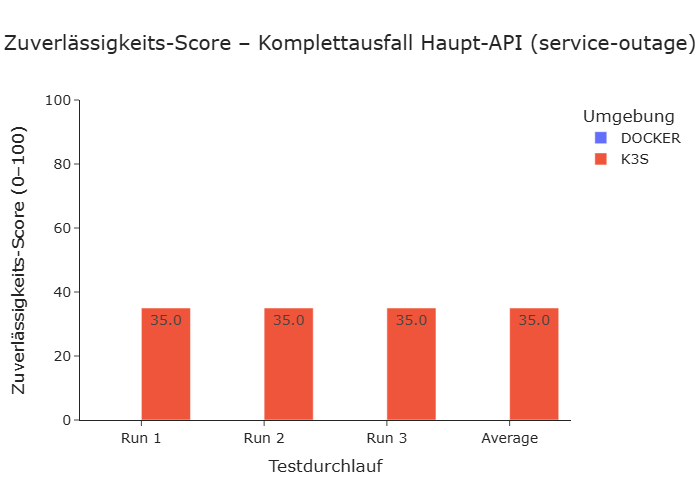
\includegraphics[width=0.8\textwidth]{bilder/tests/reliability_score_api-outage_service-outage.png}
\caption{Zuverlässigkeit Score bei Komplettausfall der Haupt-API}
\label{fig:chaos_api_outage}
\end{figure}
\FloatBarrier